\documentclass[tikz,border=12pt]{standalone}
\usepackage[T1]{fontenc}
\usepackage{mathpazo}
\usepackage{amsmath,amssymb}
\usetikzlibrary{arrows.meta, positioning, calc, fit, decorations.pathreplacing}

\definecolor{stblue}{HTML}{7B97AD}
\definecolor{rwgold}{HTML}{B8995E}
\definecolor{sage}{HTML}{7A9A7E}
\definecolor{dkbrown}{HTML}{3D3530}
\definecolor{wmgray}{HTML}{7B7067}
\definecolor{cream}{HTML}{F9F6F0}
\definecolor{border}{HTML}{D4C9B8}
\definecolor{terracotta}{HTML}{C47A6A}
\definecolor{lavender}{HTML}{907EA0}

\begin{document}
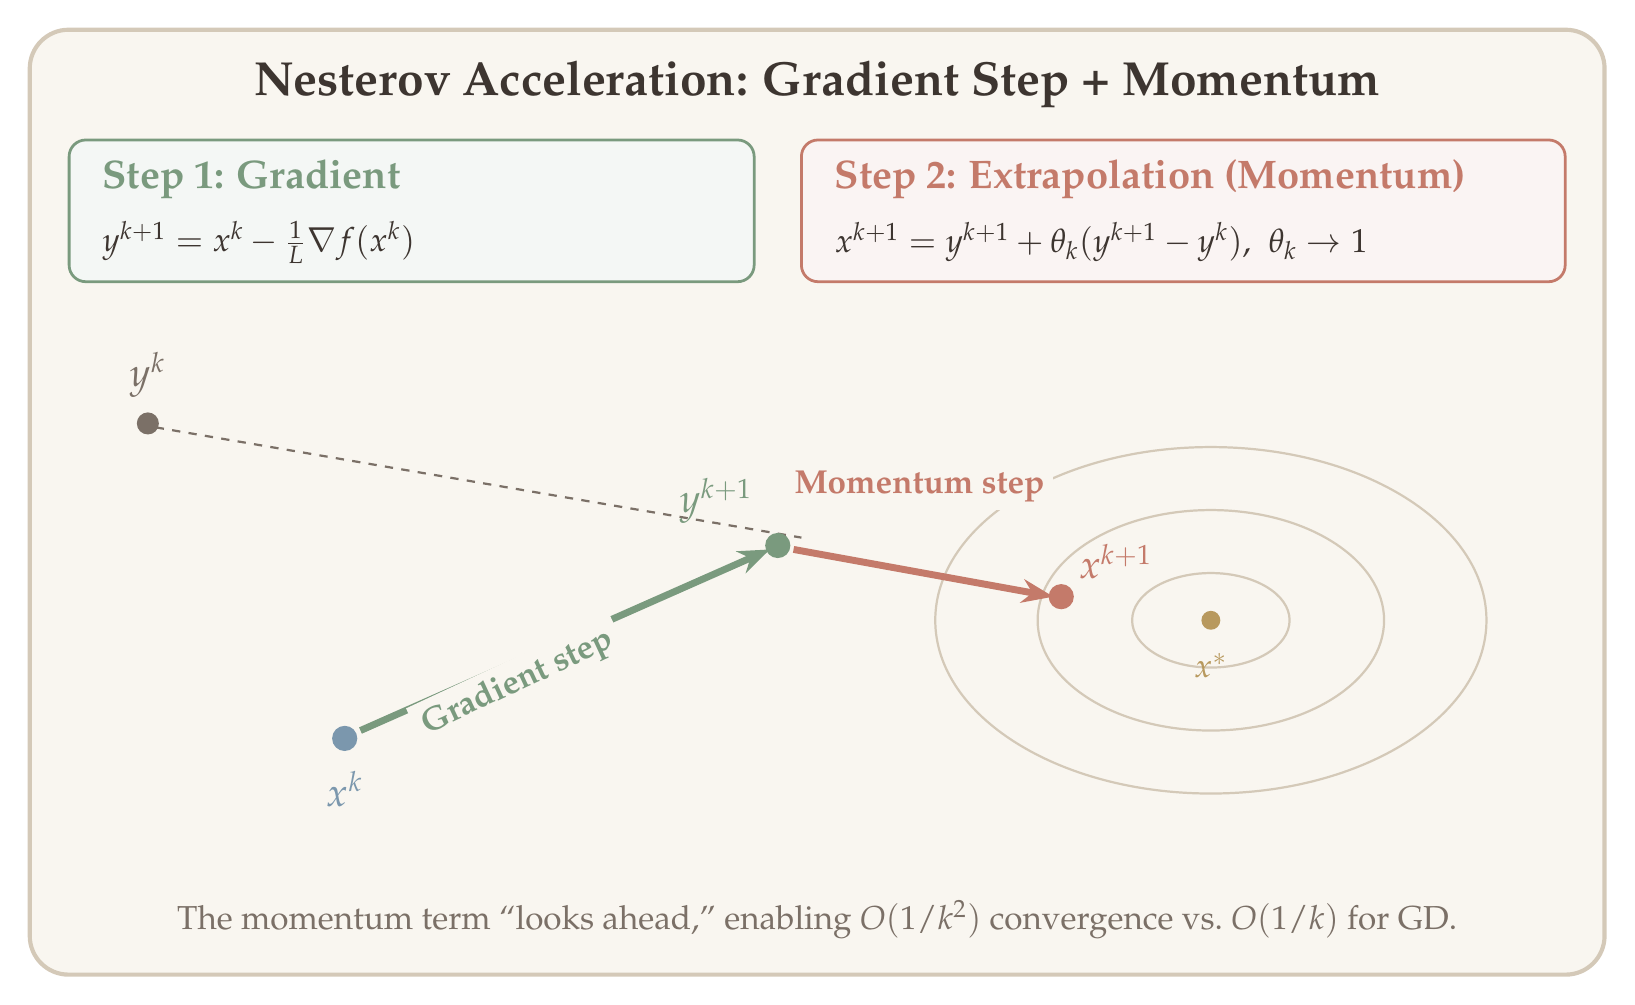
\begin{tikzpicture}[
  >={Stealth[length=4mm, width=3mm]},
  every node/.style={text=dkbrown, font=\large},
]

% Background
\fill[cream, rounded corners=14pt] (0,0) rectangle (20,12);
\draw[border, line width=1.5pt, rounded corners=14pt] (0,0) rectangle (20,12);

% Title
\node[font=\LARGE\bfseries, text=dkbrown] at (10,11.3) {Nesterov Acceleration: Gradient Step + Momentum};

% Legend boxes at top
% Step 1: Gradient
\draw[sage, line width=1pt, rounded corners=6pt, fill=sage!8]
  (0.5,8.8) rectangle (9.2,10.6);
\node[font=\Large\bfseries, text=sage, anchor=west] at (0.8,10.1) {Step 1: Gradient};
\node[font=\large, anchor=west] at (0.8,9.3) {$y^{k+1} = x^k - \tfrac{1}{L}\nabla f(x^k)$};

% Step 2: Momentum
\draw[terracotta, line width=1pt, rounded corners=6pt, fill=terracotta!8]
  (9.8,8.8) rectangle (19.5,10.6);
\node[font=\Large\bfseries, text=terracotta, anchor=west] at (10.1,10.1) {Step 2: Extrapolation (Momentum)};
\node[font=\large, anchor=west] at (10.1,9.3) {$x^{k+1} = y^{k+1} + \theta_k(y^{k+1} - y^k)$, \;$\theta_k \to 1$};

% Contour ellipses — right side
\draw[border, line width=0.8pt] (15,4.5) ellipse (3.5 and 2.2);
\draw[border, line width=0.8pt] (15,4.5) ellipse (2.2 and 1.4);
\draw[border, line width=0.8pt] (15,4.5) ellipse (1.0 and 0.6);

% Optimum
\fill[rwgold] (15,4.5) circle (0.12);
\node[font=\large, text=rwgold, below] at (15,4.2) {$x^*$};

% Point y^k (previous look-ahead) — far left
\fill[wmgray] (1.5,7.0) circle (0.14);
\node[font=\Large, text=wmgray, above] at (1.5,7.2) {$y^k$};

% Point x^k (current iterate) — left-center
\fill[stblue] (4.0,3.0) circle (0.16);
\node[font=\Large, text=stblue, below] at (4.0,2.7) {$x^k$};

% Momentum direction: dashed from y^k toward y^{k+1}
\draw[wmgray, line width=0.8pt, dashed] (1.6,6.95) -- (9.8,5.55);

% Gradient step arrow: x^k -> y^{k+1}  (long, clear)
\draw[sage, line width=2.5pt, ->] (4.2,3.1) -- (9.4,5.4);

% y^{k+1} point — center
\fill[sage] (9.5,5.45) circle (0.16);
\node[font=\Large, text=sage, above left] at (9.3,5.6) {$y^{k+1}$};

% Label for gradient step
\node[font=\large\bfseries, text=sage, fill=cream, inner sep=3pt, rotate=25]
  at (6.2,3.7) {Gradient step};

% Momentum arrow: y^{k+1} -> x^{k+1}  (clear, longer)
\draw[terracotta, line width=2.5pt, ->] (9.7,5.4) -- (13.0,4.8);

% x^{k+1} point
\fill[terracotta] (13.1,4.8) circle (0.16);
\node[font=\Large, text=terracotta, above right] at (13.2,4.9) {$x^{k+1}$};

% Label for momentum step
\node[font=\large\bfseries, text=terracotta, fill=cream, inner sep=3pt]
  at (11.3,6.2) {Momentum step};

% Bottom note
\node[font=\large, text=wmgray] at (10,0.7)
  {The momentum term ``looks ahead,'' enabling $O(1/k^2)$ convergence vs.\ $O(1/k)$ for GD.};

\end{tikzpicture}
\end{document}
